% Figure from MATH 591 notes, section 59 (Lemma: where all derivatives up to order k vanish). Added, not from lecture.
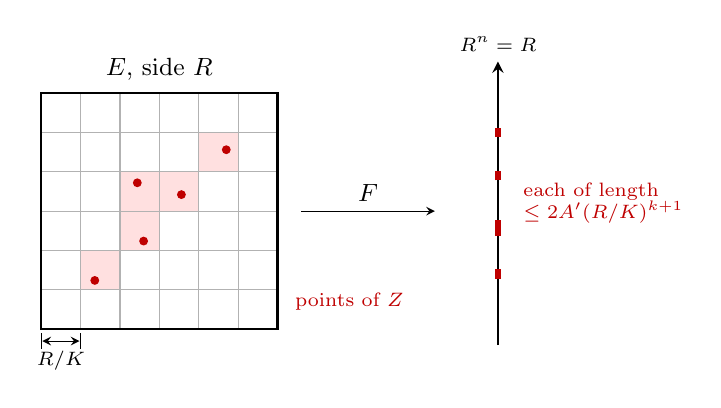
\begin{tikzpicture}[>=stealth, scale=1.0]
    \foreach \c/\r in {1/1, 2/2, 3/3, 4/4, 2/3} {
        \fill[red!12] ({0.5*\c},{0.5*\r}) rectangle ({0.5*\c+0.5},{0.5*\r+0.5});
    }
    \draw[step=0.5, gray!60] (0,0) grid (3,3);
    \draw[thick] (0,0) rectangle (3,3);
    \node[font=\small] at (1.5,3.3) {$E$, side $R$};
    \draw[|<->|] (0,-0.15) -- node[below, font=\scriptsize] {$R/K$} (0.5,-0.15);
    \foreach \x/\y in {0.68/0.62, 1.30/1.12, 1.78/1.71, 2.35/2.28, 1.22/1.86} {
        \fill[red!75!black] (\x,\y) circle (1.6pt);
    }
    \node[red!75!black, font=\scriptsize, anchor=west] at (3.1,0.35) {points of $Z$};
    \draw[->] (3.3,1.5) -- node[above, font=\small] {$F$} (5.0,1.5);
    \draw[thick, ->] (5.8,-0.2) -- (5.8,3.4) node[above, font=\scriptsize] {$\mathbb{R}^n = \mathbb{R}$};
    \foreach \y in {0.7, 1.25, 1.33, 1.95, 2.5} {
        \draw[line width=2.4pt, red!75!black] (5.8,{\y-0.06}) -- (5.8,{\y+0.06});
    }
    \node[red!75!black, font=\scriptsize, anchor=west, align=left] at (6.0,1.6) {each of length\\ $\le 2A'(R/K)^{k+1}$};
\end{tikzpicture}
